\documentclass{article}\usepackage[]{graphicx}\usepackage[]{color}
%% maxwidth is the original width if it is less than linewidth
%% otherwise use linewidth (to make sure the graphics do not exceed the margin)
\makeatletter
\def\maxwidth{ %
  \ifdim\Gin@nat@width>\linewidth
    \linewidth
  \else
    \Gin@nat@width
  \fi
}
\makeatother

\definecolor{fgcolor}{rgb}{0.345, 0.345, 0.345}
\newcommand{\hlnum}[1]{\textcolor[rgb]{0.686,0.059,0.569}{#1}}%
\newcommand{\hlstr}[1]{\textcolor[rgb]{0.192,0.494,0.8}{#1}}%
\newcommand{\hlcom}[1]{\textcolor[rgb]{0.678,0.584,0.686}{\textit{#1}}}%
\newcommand{\hlopt}[1]{\textcolor[rgb]{0,0,0}{#1}}%
\newcommand{\hlstd}[1]{\textcolor[rgb]{0.345,0.345,0.345}{#1}}%
\newcommand{\hlkwa}[1]{\textcolor[rgb]{0.161,0.373,0.58}{\textbf{#1}}}%
\newcommand{\hlkwb}[1]{\textcolor[rgb]{0.69,0.353,0.396}{#1}}%
\newcommand{\hlkwc}[1]{\textcolor[rgb]{0.333,0.667,0.333}{#1}}%
\newcommand{\hlkwd}[1]{\textcolor[rgb]{0.737,0.353,0.396}{\textbf{#1}}}%

\usepackage{framed}
\makeatletter
\newenvironment{kframe}{%
 \def\at@end@of@kframe{}%
 \ifinner\ifhmode%
  \def\at@end@of@kframe{\end{minipage}}%
  \begin{minipage}{\columnwidth}%
 \fi\fi%
 \def\FrameCommand##1{\hskip\@totalleftmargin \hskip-\fboxsep
 \colorbox{shadecolor}{##1}\hskip-\fboxsep
     % There is no \\@totalrightmargin, so:
     \hskip-\linewidth \hskip-\@totalleftmargin \hskip\columnwidth}%
 \MakeFramed {\advance\hsize-\width
   \@totalleftmargin\z@ \linewidth\hsize
   \@setminipage}}%
 {\par\unskip\endMakeFramed%
 \at@end@of@kframe}
\makeatother

\definecolor{shadecolor}{rgb}{.97, .97, .97}
\definecolor{messagecolor}{rgb}{0, 0, 0}
\definecolor{warningcolor}{rgb}{1, 0, 1}
\definecolor{errorcolor}{rgb}{1, 0, 0}
\newenvironment{knitrout}{}{} % an empty environment to be redefined in TeX

\usepackage{alltt}
\usepackage[margin=1in]{geometry}
\IfFileExists{upquote.sty}{\usepackage{upquote}}{}
\begin{document}
\title{Model Selection Metrics}
\author{Eric Reed}
\maketitle
\write18{wget https://github.com/arvindram12/Final-Project/blob/master/rank1.png}
\write18{wget https://github.com/arvindram12/Final-Project/blob/master/3crits.png}



\section{Introduction}

  The purpose of this analysis is to test three model selection metrics, Adjusted $R^2$, Aikake Information Criterion(AIC), and Bayesion information criterion (BIC), to explore how choice of these criterion can impact model selection. We will due this by building different Multiple Linear Regression Models of different combinations of predictor variables on the outcome variable, assuming linear relationships of each variable and outcome variable.  The outcome variable tesed for was systolic blood pressure.  Every model included age and sex of the study participants. The continuous variables being tested were, total cholesterol, body mass index, blood pressure, and glucose level.  The categorical variable being tested for was current smoking status, diabetes status, whether or not the participants takes blood pressure medication, and education level.

\subsection{Adjusted $R^2$}
  Adjusted $R^2$ is a selection metric that using the equation: $$R^2_a = 1-\frac{RSS/(n-p-1)}{TSS/(n-1)}$$.  Where $RSS$ is the residual sum of squares of the predictor variables, $TSS$ in the total sum of squares of the  outcome variable, $p$ is the number of predictor variables and $n$ is the number of observations.  This metic is comprable to a typical $R^2$ calculation which is simply $$R^2=1-\frac{RSS}{TSS}$$.  What is useful abou the adjusted $R^2$ however is that it may penalize added variables that don't contribute predictive value to the model.  Predictive value of a model is assessed via the Adjusted $R^2$ value as its closeness to 1.
\subsection{Aikake Information Criterion}
 The equation for Aikake Informatino Criteria is $$ AIC=nlog(RSS/n)+2(p+1)$$.  As with adjusted $R^2$, it includes the variable for residual sum of squares, numer of variables and numberof obsevations.  As is evident by apparent differences between the two equations, the AIC measures predictive value differently.  However it functions similarly that it penalizes higher values for residual sum of squares of the predictor variables and for added variable.  Also, counter to adjusted $R^2$, lower values of AIC are indicative to increased model predictive value.
 \subsection{Bayesion Information Criterion}
 The equation for Bayesian information criterion is very similar to AIC. It is $$ BIC=nlog(RSS/n)+(p+1)log(n) $$.  Here the equation are idenitical excepte for $2(p+1)$ in AIC is replaced with $(p+1)log(n)$.  Here we can see that the two metrics handle the number of observations differently.  They will therefore yeild similar but not identical values.
 
\section{Methods}
In this analysis there were 8 variables tested along with sex and age for predictive value of systolic blood pressure.  This results in 255($2^8-1$) possible combinations of variables, and therefore 255 possible multiple linear regression models, assuming linearity of every predictor variable.  These models were generated in R using the lm() function.  Lists of variables and adjusted $R^2$ were extracted directly from ``lm()" object and AIC and BIC values were calculated for each model using the ``aic()" and ``bic()" functions. respectively. As mentioned before, higher adjusted $R^2$ values and lower AIC and BIC values are indicative to model proedictive value.  The number of variables added to the model are color coded between 1 and 8.  Here, we can notice a general trend for model predictive value to increase accross all three values. However there the distribution between the AIC and BIC are much more closely related than that of the adjusted $R^2$.

\section{Results}

\begin{figure}[h]
\begin{center}
    \centering
    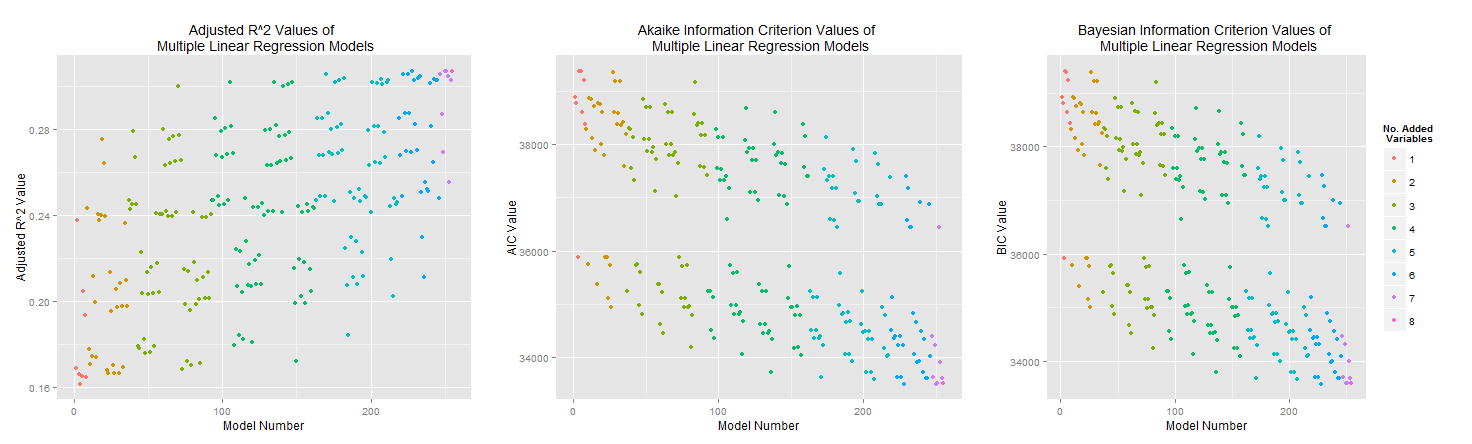
\includegraphics[width=1\textwidth]{3crits.png}
    \caption{Metric Values of MLR Models, Using Three Different  Model Selection Metrics}
    \label{fig:awesome_image}
\end{center}
\end{figure}
  
  Figure 1 depicts the output of each selection metric.  The $x-axis$ represents each of the 255 models that were gerated, and the $y-axis$ represents the respective metric value of each model.  Here we can tell that there is a broad trend for predictive value to increase as the number of added variables to increase.  However, we can see that the distribution of the adjusted $R^2$ is very different when compared to that of AIC, BIC. Since each metric will output a different value accross three of the same models it is difficult to inperpret, how the different selection metrics have ranked the models by there values alone. 
  
\begin{figure}[h]
\begin{center}
    \centering
    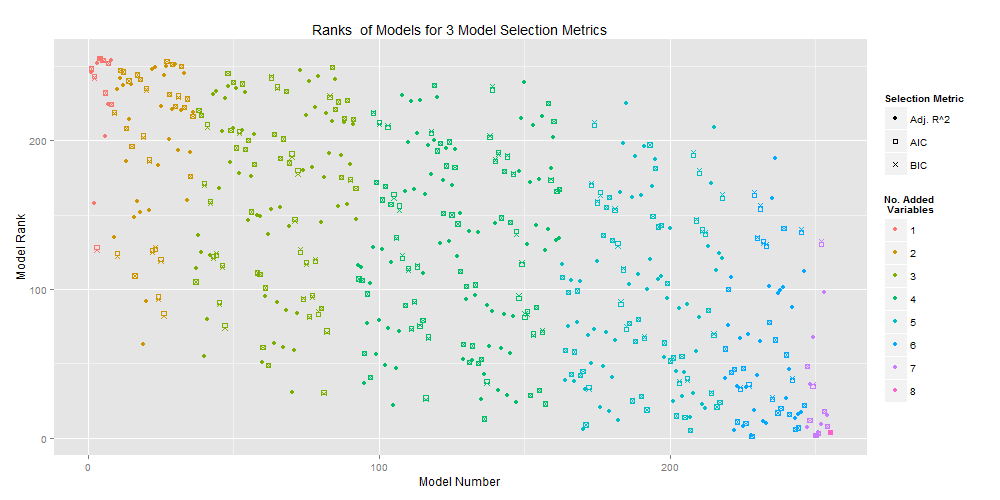
\includegraphics[width=0.8\textwidth]{rank1.png}
    \caption{Ranks of MLR Models, Using Three Different  Model Selection Metrics}
    \label{fig:awesome_image}
\end{center}
\end{figure}  
  Figure 2 represents the ranking of each model, according to each of the three selection metrics. The values of each output are ordered from strongest predictive values, 1, to weakest predictive value, 255.  Since these ranks are on the same scale we can represent all three selection metrics are now interprettable on the same graph.  The most important point here is that each metric can assign a different rank of predictive value to the same model, though AIC and BIC will more often return the same rank for a given model.

Table 1 represents the strongest predictive value for each of the number of added variables using adjusted $R^2$. Table 2 represents the strongest predictive value for each of the number of added variables using AIC and BIC.  AIC and BIC are included in the same table as they aggreed on the highest ranked model for each case. In each table the values of the other metric is given as well. 

 



\begin{table}[ht]
\begin{tiny}
\centering
\begin{tabular}{rrllllllllrrr}
  \hline
Variables & BMI & BP Med? & Heart Rt. & Tot Chol. & Glucose & Educ. & Smoke? & Diabetes & Adj $R^2$ & AIC & BIC \\ 
  \hline
        1 & YES & NO & NO & NO & NO & NO & NO & NO & 0.237966 & 38772.70 & 38804.67 \\ 
     2 & YES & YES & NO & NO & NO & NO & NO & NO & 0.275382 & 38006.02 & 38044.29 \\ 
     3 & YES & YES & YES & NO & NO & NO & NO & NO & 0.300141 & 37844.80 & 37889.45 \\ 
     4 & YES & YES & YES & YES & NO & NO & NO & NO & 0.301882 & 37398.21 & 37449.15 \\ 
     5 & YES & YES & YES & YES & YES & NO & NO & NO & 0.30543 & 34387.96 & 34444.50 \\ 
     6 & YES & YES & YES & YES & YES & YES & NO & NO & 0.306995 & 33499.77 & 33574.84 \\ 
     7 & YES & YES & YES & YES & YES & YES & YES & NO & 0.307125 & 33500.04 & 33581.37 \\ 
     8 & YES & YES & YES & YES & YES & YES & YES & YES & 0.306962 & 33501.94 & 33589.52 \\  
   \hline
   \end{tabular}
\caption{Multiple Linear Regression Models for Maximum Adjusted $R^2$}
\end{tiny}
\end{table}

   \begin{table}[ht]
   \begin{tiny}
\centering
\begin{tabular}{rrlllllllllrr}
  \hline
  Variables & Glucose & Educ. & BP Med? & BMI & Heart Rate & Tot Chol. & Smoke? & Diab. & Adj $R^2$ & AIC & BIC \\ 
  \hline
  1 & YES & NO & NO & NO & NO & NO & NO & NO & 0.237966 & 38772.70 & 38804.67 \\ 
     2 & YES & YES & NO & NO & NO & NO & NO & NO & 0.275382 & 38006.02 & 38044.29 \\ 
     3 & YES & YES & YES & NO & NO & NO & NO & NO & 0.300141 & 37844.80 & 37889.45 \\ 
     4 & YES & YES & YES & YES & NO & NO & NO & NO & 0.301882 & 37398.21 & 37449.15 \\ 
     5 & YES & YES & YES & YES & YES & NO & NO & NO & 0.30543 & 34387.96 & 34444.50 \\ 
     6 & YES & YES & YES & YES & YES & YES & NO & NO & 0.306995 & 33499.77 & 33574.84 \\ 
     7 & YES & YES & YES & YES & YES & YES & YES & NO & 0.307125 & 33500.04 & 33581.37 \\ 
     8 & YES & YES & YES & YES & YES & YES & YES & YES & 0.306962 & 33501.94 & 33589.52 \\ 
   \hline
\end{tabular}
\caption{Multiple Linear Regression Models for Minimum AIC and BIC}
\end{tiny}
\end{table}

The main trend that every metric followed was that once a variable was added to the model, it was present in each of the following models, when a new variable was added.  For example, in the case of adjusted $R^2$ BMI was demonstrated to be the best single added variable predictor. Next, blood pressure medication status was added along with BMI to be the strongest two added variable predictors.  These two were also present in the strongest 3 added variable predictors along with heart rate.  

Ultimately the strongest model as predicted by adjusted $R^2$ differed from AIC and BIC by one variable. The strongest model predicted by adjusted $R^2$, in order of added variables was: BMI, blood pressure medication, heart rate, total cholesterol, glucose, education, and smoking status, while that predicted by AIC and BIC in order of added variables was: glucose, education, blood pressure medication, BMI, heart rate, and total cholesterol. Therefore, the addition of smoking status by adjusted $R^2$ and the lack there of in AIC and BIC is the only difference between the  strongest presumed model.

What's perhaps most striking is that if we were to try and use these same variables to predict the strongest model by adding less than 6 variables, than adjusted $R^2$ and AIC, and BIC would have yielded different models entirely.  For example the strongest three added variable predictor by adjusted $R^2$ was BMI, blood pressure medication, and heart rate,  while that of AIC and BIC was glucose, education, and blood pressure medication.



\end{document}
